
%%%
%%% CHAPTER
%%%
\chapter{Second Law of Thermodynamics}\label{Chapter:FirstLaw}

   \begin{LearningObjectivesBlock}{Learning Objectives}
      Upon completion of this chapter, you will be able to
        \begin{enumerate}
           \item Demonstrate understanding of key concepts of entropy and the second law of thermodynamics;
           \item Apply first and second laws of thermodynamics to assess of heat transfer and process reversibility;
           \item Know that Clausius inequality is an alternative statement of the second law;
           \item Demonstrate how to apply the entropy balance in a thermodynamic system;
           \item Recognise processes that generate entropy.
        \end{enumerate}
\medskip
     Recommended reading: Chapters 5 of \citet{SmithVanNess_Book,Moran_Book,Borgnakke_Book} or 3 of \citet{Atkins_Book}.
   \end{LearningObjectivesBlock}


  
%%%
%%% SECTION
%%%
   \section{Introduction}\label{Chapter:SecondLaw:Section:Intro}
   The first law (Chapters~\ref{Chapter:Introduction} and \ref{Chapter:FirstLaw}) demonstrated that energy can flow either from or to a system in the form of heat or work, however it does not indicate the direction of process (\ie energy flow). The second law of thermodynamics concerns about feasibility, direction and spontaneity of processes and entropy..
   
The second law of thermodynamics is a general principle which makes constraints upon spontaneity of the process, direction of heat transfer and general efficiency of heat engines, \eg a hot body cools to the temperature of the surroundings or a chemical reaction that may run in one direction instead of the reverse (\eg combustion of ethane producing carbon dioxide and water). The reverse of such processes may occur but they will not be spontaneous.  
  
%%%
%%% SECTION
%%%
   \section{Statement of the Second Law}\label{Chapter:SecondLaw:Section:SecondLawStatement}\index{Laws of Thermodynamics ! Second law}
The second law of thermodynamics was stated separately by \citet{Clausius_Book}, Kelvin \citep{Thomson_1851} and \citet{Planck_Book} in slightly different ways. Each statement is based on irreversible processes.
\begin{shaded}
  \begin{center}
    {\bf Clausius Statement}
  \end{center}
  'It is impossible for a self-acting machine working in a cyclic process unaided by any external agency, to convey heat from a body at a lower temperature to a body at a higher temperature.'
\end{shaded}
This statement clearly indicates that heat cannot spontaneously flow from a colder to a hotter body. This can only be realised if other effects play some role, \eg in a refrigeration process in which external work is used to extract heat from low temperature body and reject it into a high temperature body (Fig.~\ref{Chapter:SecondLaw:Fig:SecondLawStatement})

   %%% FIGURE
   \begin{figure}[h]
     \begin{center}
        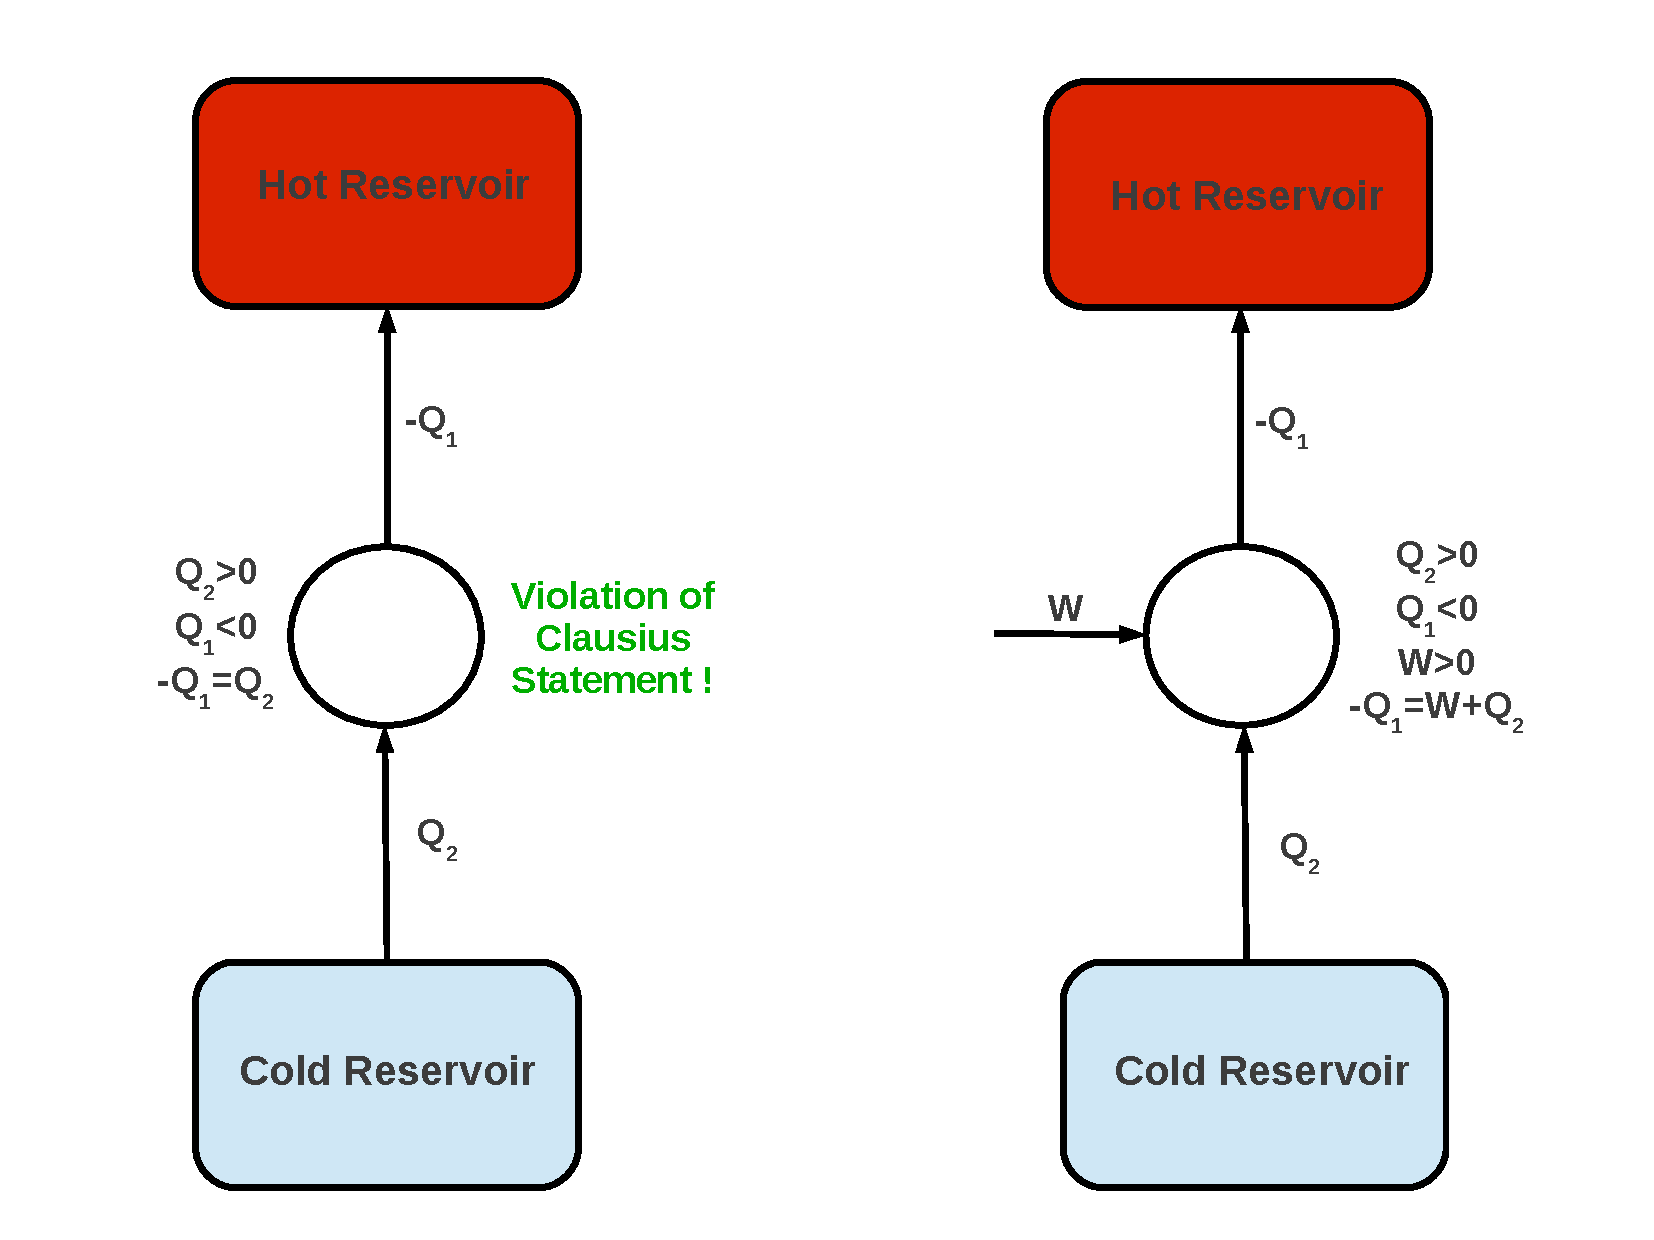
\includegraphics[width=.8\columnwidth,clip]{./Figs/2ndLaw_Schem}
     \caption{All spontaneous processes are irreversible -- heat flows from hot to cold spontaneously and irreversibly. }\label{Chapter:SecondLaw:Fig:SecondLawStatement}
     \end{center}
   \end{figure} 

\begin{shaded}
  \begin{center}
    {\bf Kelvin-Planck Statement}
  \end{center}
  'It is impossible to construct an engine, which while operating in a cycle produces no other effect except to extract heat from a single reservoir and do equivalent amount of work.'
\end{shaded}
This statement indicates that in order to achieve net work from a heat engine (\ie a device operating in cycle), there should be heat interaction between two bodies (\ie thermal reservoirs) at different temperatures (\ie thermal source or sink). 

   
   % Example
   \begin{MyExample}{\begin{center}{\bf Example}\end{center}}
     \begin{example}\label{Chapter:SecondLaw:Example1}\citep{Rajput_Book}
        A heat engine receives heat at the rate of 1500 kJ.min$^{-1}$ and gives an output of 8.2 kW. Determine:
        \begin{enumerate}[a)]
          \item Thermal efficiency;
          \item Rate of heat rejection $\left(\text{in kJ.s}^{-1}\right)$.
        \end{enumerate}
     \end{example}

% SOLUTION
       \noindent{\bf Solution:}
       The heat received by the engine (Fig.~\ref{Chapter:FirstLaw:Fig:PowerRefrigSystems}) is $Q_{1}=$ 1500 kJ.min$^{-1}$ = 25 kJ.s$^{-1}$, and the output work is $W=$ 8.2 kW = 8.2 kJ.s$^{-1}$. Thus
       \begin{enumerate}[a)]
         \item the thermal efficiency is defined as (Eqn.~\ref{Chapter:FirstLaw:Eqn:FirstLawCycle:PowerEfficiency}),
           \begin{displaymath}
             \eta_{\text{th}} = \frc{W}{Q_{1}} = 0.3280 \;\;\Longrightarrow\;\; 32.80\%;
           \end{displaymath}
         \item the rate of heat rejection is effectively a result of the energy balance on the system,
           \begin{displaymath}
             Q_{2}=Q_{1}-W = 16.80 \text{ kJ.s}^{-1}
           \end{displaymath}
           
       \end{enumerate}
   \end{MyExample}
   
   % Example
   \begin{MyExample}{\begin{center}{\bf Example}\end{center}}
     \begin{example}\label{Chapter:SecondLaw:Example2}\citep{Rajput_Book}
        A domestic food refrigerator maintains a temperature of -12$^{\circ}$C. The ambient air temperature is 35$^{\circ}$C. If heat leaks into the freezer at the continuous rate of 2 kJ.s$^{-1}$, determine the least power necessary to pump this heat out continuously.
     \end{example}

% SOLUTION
       \noindent{\bf Solution:}
       For freezer and ambient temperatures of 261.15 K and 308.15 K and assuming reversible process (see Eqn.~\ref{Chapter:FirstLaw:Eqn:FirstLawCycle:PowerEfficiency2}) based on the energy balance of the refrigeration cycle (Fig.~\ref{Chapter:FirstLaw:Fig:PowerRefrigSystems}b), 
       \begin{displaymath}
          \frc{Q_{2}}{Q_{1}} = \frc{T_{2}}{T_{1}} \;\;\Longrightarrow \;\;Q_{1} = \frc{Q_{2}}{T_{2}}T_{1} = \frc{2.00}{261.15}\times 308.15 = 2.3599\text{ kJ.s}^{-1},
       \end{displaymath}
       where $Q_{2}$ and $Q_{1}$ are the heat flowing from the cold reservoir and to the hot reservoir, respectively. Now, calculating the power (based on the energy balance in the system)
       \begin{displaymath}
          W = Q_{1}-Q_{2} = 0.3599\text{ kJ.s}^{-1}.
       \end{displaymath}
   \end{MyExample}
   

%%%
%%% SECTION
%%%
   \section{Mathematical Statement of the Second Law}\label{Chapter:SecondLaw:Section:SecondLawStatement_Maths}\index{Laws of Thermodynamics ! Second law}
     \begin{subequations}
        In Fig.~\ref{Chapter:SecondLaw:Fig:SecondLawStatement2}, an infinitesimal amount of heat, $\delta Q^{\prime}$, is transferred from the thermal reservoir (with temperature $T_{res}$) to a reversible cyclic engine (1). The engine produces a small amount of work, $\delta W^{\prime}$, and releases an infinitesimal amount of heat, $\delta Q$ to another reservoir (at variable temperature $T$) that also releases energy in form of work $\left(\delta W\right)$ to the surroundings.

%%% FIGURE
   \begin{figure}[h]
     \begin{center}
        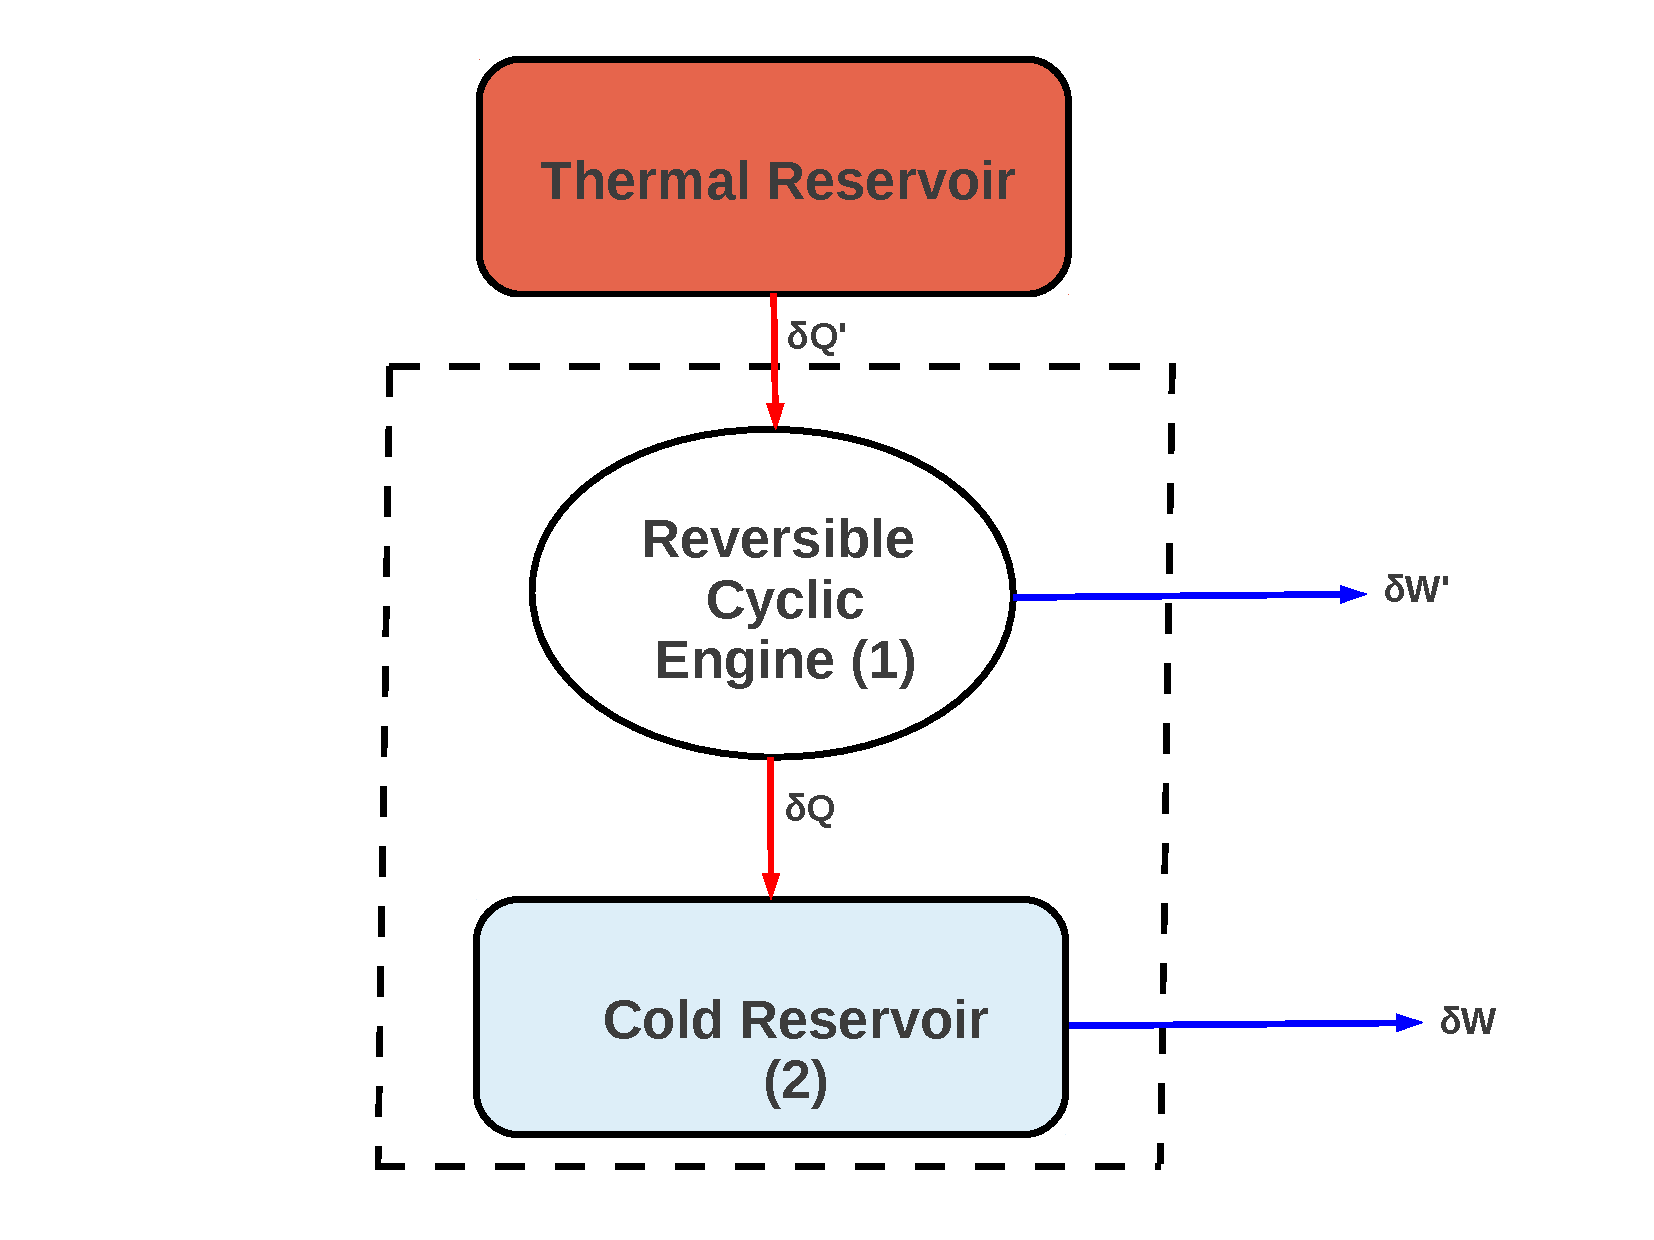
\includegraphics[width=.8\columnwidth,clip]{./Figs/2ndLaw_Schem2}
     \caption{Thermal power device for mathematical derivation of the Second law. }\label{Chapter:SecondLaw:Fig:SecondLawStatement2}
     \end{center}
   \end{figure} 

        Using the analogy of heat transfer ratio and temperature ratio (see power cycle systems in Section~\ref{Chapter:FirstLaw:Section:FirstLaw_Cycle}),
           \begin{displaymath}
              \frc{\delta Q^{\prime}}{\delta Q} = \frc{T_{res}}{T} \;\; \Longrightarrow \frc{\delta Q^{\prime}}{T_{res}} = \frc{\delta Q}{T}.
           \end{displaymath}
        An energy balance (in differential form) for the combined cycle (within the dotted box) is
           \begin{eqnarray}
              && dU = \text{Energy In} - \text{Energy Out} \nonumber \\
              && dU = \delta Q^{\prime} - \left(\delta W + \delta W^{\prime}\right) \Longrightarrow \delta W + \delta W^{\prime} = \delta Q^{\prime} - dU. \nonumber 
           \end{eqnarray}
        Note that the first law is explicitly applied in the second equation above using the sign convention (\ie energy removed from the system is negative whereas energy added to the system is positive). The process is not required to be cyclic and the heat transfer $\delta Q$ is internal and does not cross the boundaries of the combined system. Thus, eliminating $\delta Q^{\prime}$,
           \begin{displaymath}
              \delta W + \delta W^{\prime} = T_{res}\frc{\delta Q}{T} - dU.
           \end{displaymath}
        If the power configuration undergoes a cyclic process,
           \begin{displaymath}
              \oint\delta W + \oint\delta W^{\prime} = \oint T_{res}\frc{\delta Q}{T} -\oint dU,
           \end{displaymath}
        and as $U$ is a thermodynamic property, the cyclic integral is equal to zero.  Integrating the equation above, and assuming that $T_{res}$ is (by definition) constant,
           \begin{displaymath}
              W + W^{\prime} = T_{res}\oint \frc{\delta Q}{T}. 
           \end{displaymath}
        From Kelvin-Planck statement of the Second Law, not all heat can be converted into work, but all work can be converted into heat, thus $W + W^{\prime}\le 0$ (\ie work is always produced in a power cycle and exported to the surroundings) and therefore 

       \begin{shaded}
           \begin{displaymath}
             T_{res}\oint \frc{\delta Q}{T} \le 0.\label{Chapter:SecondLaw:Eqn:SecondLawMathExpression1}
           \end{displaymath}
           Since $T_{res}>0$ (absolute temperature), this integral equation can be divided by $T_{res}$ without changing the meaning of the inequality to obtain the mathematical representation of the Second Law,
           \begin{equation}
             \begin{cases}
                \displaystyle\oint\frc{\delta Q}{T} < 0, & \;\;\text{ for irreversible processes} \\
                \displaystyle\oint\frc{\delta Q}{T} = 0, & \;\;\text{ for reversible processes} 
             \end{cases}\label{Chapter:SecondLaw:Eqn:SecondLawMathExpression2}
           \end{equation}
           This is called {\bf Clausius inequality}.\index{Clausius inequality}
       \end{shaded}
     \end{subequations}

%%%
%%% SECTION
%%%
   \section{Entropy}\label{Chapter:SecondLaw:Section:Entropy}\index{Laws of Thermodynamics ! Second law}
     \begin{subequations}
       Let's consider the reversible process shown in Fig.~\ref{Chapter:Introduction:Fig:CyclesSchematic}, from state 1 to 2, via path {\it A}, and returning to state 2 from either path {\it B} or {\it C}. The Clausius inequality, $\displaystyle\oint\frc{\delta Q}{T} = 0$, can be split as,
           \begin{displaymath}
             \begin{cases}
                \left(\displaystyle\int_{1}^{2}\frc{\delta Q}{T}\right)_{A} + \left(\displaystyle\int_{2}^{1}\frc{\delta Q}{T}\right)_{B} = 0, \\
                \left(\displaystyle\int_{1}^{2}\frc{\delta Q}{T}\right)_{A} + \left(\displaystyle\int_{2}^{1}\frc{\delta Q}{T}\right)_{C} = 0,
             \end{cases}
           \end{displaymath}
       leading to,
           \begin{displaymath}
                \left(\displaystyle\int_{2}^{1}\frc{\delta Q}{T}\right)_{B} = \left(\displaystyle\int_{2}^{1}\frc{\delta Q}{T}\right)_{C} = 0.
           \end{displaymath}
           Since paths {\it B} and {\it C} are different and arbitrary, but $\displaystyle\int\limits_{2}^{1}\displaystyle\frac{\delta Q}{T}$ is the same on either paths -- therefore {\bf the integral is path-independent}. 
           \begin{shaded}
               This defines another thermodynamic property, the {\bf entropy}\index{Entropy},
               \begin{equation}
                  S_{2}-S_{1} = \displaystyle\int_{1}^{2}\frc{\delta Q}{T}.\label{Chapter:SecondLaw:Eqn:Entropy}
               \end{equation}
           \end{shaded}
          Assuming constant mass ($m$), the intensive property entropy $\left(s=S/m\right)$, the differential form is, 
           \begin{displaymath}
                ds = \frc{\delta q}{T} \;\;\;\; \Longrightarrow \;\;\;\; \delta q = Tds,
           \end{displaymath}
           which is the heat transfer equivalent of 
           \begin{displaymath}
                \delta w = \displaystyle\int_{1}^{2}PdV.
           \end{displaymath}
 
           For a reversible process,
           \begin{displaymath}
                S_{2} - S_{1} = \displaystyle\int\limits_{1}^{2}\frc{\delta Q}{T}\;\;\text{ and } \;\; S_{1} - S_{2} = \displaystyle\int\limits_{2}^{1}\frc{\delta Q}{T},
           \end{displaymath}
           and from the Second law
           \begin{displaymath}
                0 \geq \left( \displaystyle\int\limits_{1}^{2}\frc{\delta Q}{T} \right)_{A} + \left( \displaystyle\int\limits_{2}^{1}\frc{\delta Q}{T} \right)_{B}.
           \end{displaymath}
       \begin{shaded}
           These integral expressions can be combined to eliminate path $B$ and obtain a general expression of entropy of arbitrary processes
           \begin{displaymath}
                dS = S_{2}-S_{1} \geq \displaystyle\int\limits_{1}^{2}\frc{\delta Q}{T}
           \end{displaymath}
           where
           \begin{displaymath}
               dS
                \begin{cases}
                      = \frc{dQ}{T} & \;\;\text{ for reversible processes} \\
                      > \frc{dQ}{T} & \;\;\text{ for irreversible processes}.
                \end{cases}
           \end{displaymath}           
       \end{shaded}
     \end{subequations}


%%%
%%% SECTION
%%%
   \section{Entropy Changes}\label{Chapter:SecondLaw:Section:EntropyChanges}
     \begin{subequations}
       From the First Law equation,
           \begin{displaymath}
              dU = dQ - PdV
           \end{displaymath} 
           If we differentiate the enthalpy equation -- $H = U + PV$.
                \begin{displaymath}
                    dH = dU + d(PV) = dU + PdV +VdP,
                \end{displaymath}
           and replace the previous equation,
                \begin{displaymath}
                    dH - \cancel{PdV} - VdP = dQ - \cancel{PdV} \;\;\Rightarrow \;\; dQ = dH - VdP
                \end{displaymath}
           For {\it ideal gas}, $C_{p}^{\text{ig}}=\left(\frac{dH}{dT}\right)_{P}$ and $V=\frc{RT}{P}$,
                \begin{eqnarray}
                  dQ &=& C_{p}^{\text{ig}} dT - \frc{RT}{P}dP\;\;\;\;\;\times\left(\frc{1}{T}\right) \nonumber \\
                  \frc{dQ}{T} &=& \frc{C_{p}^{\text{ig}}}{T}dT - \frc{R}{P}dP \nonumber \\
                  dS &=& \frc{C_{p}^{\text{ig}}}{T}dT - \frc{R}{P}dP, \nonumber
                \end{eqnarray}
           where $S$ is the molar entropy of ideal gas. 
           \begin{shaded}
              Integrating from state 0 to state 1,
                \begin{eqnarray}
                    \int\limits_{S_{0}}^{S_{1}} dS &=& \int\limits_{T_{0}}^{T_{1}} \frc{C_{p}^{\text{ig}}}{T}dT - R\int\limits_{P_{0}}^{P_{1}}\frc{dP}{P} \nonumber \\
                    \left(S_{1}-S_{0}\right) &=& \int\limits_{T_{0}}^{T_{1}} \frc{C_{p}^{\text{ig}}}{T}dT - R\ln{\frc{P_{1}}{P_{0}}} \;\;\;\;\times\left(\frc{1}{R}\right) \nonumber \\
                    \frc{\Delta S}{R} &=& \int\limits_{T_{0}}^{T_{1}} \frc{C_{p}^{\text{ig}}}{R}\frc{dT}{T} - \ln{\frc{P_{1}}{P_{0}}}.\label{Chapter:SecondLaw:Eqn:EntropyChanges1}
                \end{eqnarray}
                Although this equation was derived for mechanically reversible processes, it focuses on \underline{properties only} and is independent of the process. Thus it can be used to calculate entropy changes of {\it ideal gases}. A similar expression can be obtained as a function of $C_{v}$,
                \begin{equation}
                   \frc{\Delta S}{R} = \int\limits_{T_{0}}^{T_{1}} \frc{C_{v}}{R}\frc{dT}{T} +  \ln{\frc{V_{1}}{V_{0}}}\label{Chapter:SecondLaw:Eqn:EntropyChanges2}
                \end{equation}               
           \end{shaded}


   \begin{MyExample}{\begin{center}{\bf Example}\end{center}}
     \begin{example}\label{Chapter:SecondLaw:Example3}\citep{SmithVanNess_Book}
       For an ideal gas with constant heat capacity undergoing a reversible adiabatic (and therefore isentropic) process, Eqn.~\ref{Chapter:FirstLaw:Eqn:AdiabaticProcesses_TPGamma} can be written as
         \begin{displaymath}
             \frc{T_{2}}{T_{1}} = \left(\frc{P_{2}}{P_{1}}\right)^{\frac{\gamma-1}{\gamma}}.
         \end{displaymath}
         Show that these same equation results from application of Eqn.~\ref{Chapter:SecondLaw:Eqn:EntropyChanges1} with $\Delta S=$ 0.
     \end{example}

% SOLUTION
       \noindent{\bf Solution:} As $C_{p}^{\text{ig}}$ is constant and different from zero, Eqn.~\ref{Chapter:SecondLaw:Eqn:EntropyChanges1} can be rewritten as
          \begin{displaymath}
             \Delta S = 0 = \ln{\frc{T_{2}}{T_{1}}} - \frc{R}{C_{p}^{\text{ig}}}\ln{\frc{P_{2}}{P_{1}}}.
          \end{displaymath}
           Using Eqn.~\ref{Chapter:FirstLaw:Eqn:HeatCapacitiesRelation_IdealGas1} for an ideal gas with $\gamma = \frac{C_{p}^{\text{ig}}}{C_{v}^{\text{ig}}}$ (Eqn.~\ref{Chapter:FirstLaw:Eqn:HeatCapacitiesRelation1}):
          \begin{displaymath}
             C_{p}^{\text{ig}} = C_{v}^{\text{ig}} + R \;\;\Longrightarrow\;\; \frc{R}{C_{v}^{\text{ig}}} = \frc{\gamma-1}{\gamma},
          \end{displaymath}
          leading to
          \begin{displaymath}
             \Delta S = 0 = \ln{\frc{T_{2}}{T_{1}}} = \frc{\gamma-1}{\gamma}\ln{\frc{P_{2}}{P_{1}}} \;\;\Longrightarrow \;\; \frc{T_{2}}{T_{1}} = \left(\frc{P_{2}}{P_{1}}\right)^{\frac{\gamma-1}{\gamma}}
          \end{displaymath}

   \end{MyExample}


           \begin{shaded}
             Other important entropy relations for {\it any} gas:
             \begin{enumerate}[a)]
                \item Heating a gas at constant volume:
                  \begin{equation}
                    dS = C_{v}\frc{dT}{T}\label{Chapter:SecondLaw:Eqn:EntropyChanges3}
                  \end{equation}
                \item Heating a gas at constant pressure:
                  \begin{equation}
                    dS = C_{p}\frc{dT}{T}\label{Chapter:SecondLaw:Eqn:EntropyChanges4}
                  \end{equation}
                \item Isothermal process:
                  \begin{equation}
                    dS = R\frc{dV}{V}\label{Chapter:SecondLaw:Eqn:EntropyChanges5}
                  \end{equation}
                \item Adiabatic process (reversible):
                  \begin{equation}
                    dS = 0\label{Chapter:SecondLaw:Eqn:EntropyChanges6}
                  \end{equation}
             \end{enumerate}            
           \end{shaded}
           
     \end{subequations}

  
   % Example
   \begin{MyExample}{\begin{center}{\bf Example}\end{center}}
     \begin{example}\label{Chapter:SecondLaw:Example4}\citep{Singh_Book}
        Calculate the change in entropy of air $\left(\text{in kJ.kg}^{-1}\text{.K}^{-1}\right)$, if it is throttled (\ie isenthalpic process, or in other words at constant enthalpy) from 5 bar, 27$^{\circ}$C to 2 bar adiabatically. Given $C_{p}=$ 1.004 kJ.(kg.K)$^{-1}$, $R=$ 8.3145 J.(mol.K)$^{-1}$. Assume ideal gas behaviour and the molar mass of air is 29 g.mol$^{-1}$.
     \end{example}

% SOLUTION
       \noindent{\bf Solution:}
       \begin{center}
          \begin{tabular}{l c l}
             $P_{1}=$ 5 bar     &                           & $P_{2}=$ 2 bar \\
                               & \;\;$\Longrightarrow$\;\; &                \\
             $T_{1}=$ 300.15 K  &                           & $T_{2}$
       \end{tabular}
       \end{center}
       As there is no information \wrt the type of process, we can not assume a reversible adiabatic process, in which $\Delta S=$ =0. Therefore, we could use Eqn.~\ref{Chapter:SecondLaw:Eqn:EntropyChanges1} to calculate $\Delta S$, 
       \begin{displaymath}
          \frc{\Delta S}{R} = \frc{C_{p}^{\text{ig}}}{R}\ln{\frc{T_{2}}{T_{1}}} - \ln{\frc{P_{2}}{P_{1}}},
       \end{displaymath}
       although we do not know $T_{2}$. However, the expansion occurs isenthalpically, \ie 
       \begin{eqnarray}
            h_{1} &=& h_{2} \nonumber \\
            C_{p}^{\text{ig}}T_{1} &=& C_{p}^{\text{ig}}T_{2} \nonumber \\
            T_{1} &=& T_{2}, \nonumber
       \end{eqnarray}
       thus,
       \begin{eqnarray}
          \Delta S &=& C_{p}^{\text{ig}}\ln{\frc{T_{2}}{T_{1}}} - R\ln{\frc{P_{2}}{P_{1}}} \nonumber \\
                   &=& 0.2627\text{ J.g}^{-1}\text{.K}^{-1} = 0.2627\text{ kJ.kg}^{-1}\text{.K}^{-1} \nonumber
       \end{eqnarray}
   \end{MyExample}

   % Example
   \begin{MyExample}{\begin{center}{\bf Example}\end{center}}
     \begin{example}\label{Chapter:SecondLaw:Example5}\citep{SmithVanNess_Book}
         A rigid vessel of volume of 0.06 m$^{3}$ contains an ideal gas with $C_{v}=\frac{5}{2}R$, at 500 K and 1 bar. If 15 kJ of heat is transferred to the gas, determine the entropy of change $\left(\text{in J.K}^{-1}\right)$.
     \end{example}

% SOLUTION
       \noindent{\bf Solution:} 
            We can use Eqn.~\ref{Chapter:SecondLaw:Eqn:EntropyChanges2} to calculate the entropy change,
               \begin{displaymath}
                  \Delta S = C_{v}\ln{\frc{T_{2}}{T_{1}}} + R\ln{\frc{V_{2}}{V_{1}}},
               \end{displaymath}
               as the process take place in a rigid vessel, $V_{2}=V_{1}$, and the second term vanishes. However, in order to obtain the entropy change, $T_{2}$ must be calculated. As the volume is kept constant, there is no work produced or received by the system, $\delta W=$ 0, thus
              \begin{eqnarray}
                  \Delta U = \delta Q = 15000\text{ J} &=& C_{v}\left(T_{2}-T_{1}\right) =  \frc{5}{2}R\left(T_{2}-T_{1}\right) \nonumber \\
                                                       &=& \frc{5}{2} \times 8.3145\text{ J.mol}^{-1}\text{.K}^{-1}\left(T_{2}- 500\right)\text{ K}. \nonumber  
              \end{eqnarray}
              From the expression above, it is clear that there is an unbalance on the units as the right-hand side results in J.mol$^{-1}$ whereas the left-hand side is in J. This can be fixed by multiplying the right-hand side by the total number of moles in the vessel (\ie total energy of the system rather than the energy per mole), which can be easily calculated from the initial conditions using the ideal gas equation of state:  
              \begin{displaymath}
                  n = \frc{P_{1}V_{1}}{RT_{1}} = \frc{1\text{ bar}\times 0.06\text{ m}^{3}}{8.3145\times 10^{-5}\text{ bar.m}^{3}\text{.mol.K}^{-1} \times 500\text{ K}} = 1.4432\text{ moles}.
              \end{displaymath}
              Hence, $T_{2}=$ 1000.02 K. Now, using Eqn.~\ref{Chapter:SecondLaw:Eqn:EntropyChanges2}
               \begin{displaymath}
                  \Delta S = C_{v}\ln{\frc{T_{2}}{T_{1}}} + \cancelto{0}{R\ln{\frc{V_{2}}{V_{1}}}} = 14.4083\text{ J.mol}^{-1}\text{.K}^{-1}.
               \end{displaymath}
              $\Delta S$ can be converted to J.K$^{-1}$ by multiplying it by the number of moles, leading to 20.7941 J.K$^{-1}$.

   \end{MyExample}

   
\clearpage   
\begin{FinalSummaryBlock}{Summary}
    \begin{itemize}
       \item Clausius inequality:
            \begin{displaymath}
                \displaystyle\int \frc{\delta Q}{T} \le 0
            \end{displaymath}
       \item Both statements of the Second law establish that in order to achieve net work from a device operating in cycle, there should be heat interaction between the thermal reservoirs;
       \item 
           \begin{displaymath}
               dS
                \begin{cases}
                      = \frc{dQ}{T} & \;\;\text{ for reversible processes} \\
                      > \frc{dQ}{T} & \;\;\text{ for irreversible processes}.
                \end{cases}
           \end{displaymath}
    \end{itemize}
\end{FinalSummaryBlock}
